\clearpage
\section{Übersicht Lösungsideen}
\subsection{Idee 1}
\begin{figure}[h!]
	\centering
	\includegraphics[scale=0.75]{../../fig/Wurfmaschine_Drehraeder.png}
	\caption{Aufbau mit zwei Rädern}
	\label{fig:konzept1}
\end{figure}
Durch die Technologierecherchen im Internet wurde sehr schnell eine erste Idee gefunden. Die Bälle werden durch Einklemmen zwischen zwei entgegengesetzt drehenden Rädern in Drehrichtung beschleunigt.

\subsection{Idee 2}
\begin{figure}[h!]
	\centering
	\includegraphics[width=0.8\textwidth]{../../fig/Springer.jpg}
	\caption{Sprungfähiges Gefährt}
	\label{fig:springer}
\end{figure}
Auch die zweite Idee beruht auf einer schon bestehenden Technologie. Analog dem "SandFlea" genannten Roboter von Boston Dynamics, wäre die Maschine fähig in die Luft zu springen. Die Bälle könnten während dem gesamten Ablauf im Gerät verbleiben, da der Roboter mitsamt Bällen in den Korb springen würde.

\newpage
\subsection{Idee 3}
\begin{figure}[h!]
	\centering
	\includegraphics[width=0.4\textwidth]{../../fig/Druckluftrohr.jpg}
	\caption{Druckluftrohr}
	\label{fig:druckluftrohr}
\end{figure}
Bei der dritten Idee wird das Wurfgeschoss mittels einer schnellen Druckbeaufschlagung durch Druckluft beschleunigt. Jeweils ein Ball wird in ein einseitig offenes Rohr mit einem Ventil am geschlossenen Ende gelegt. Bei einem schlagartigen Öffnen, des an ein Druckluftsystem angeschlossenen Ventiles, strömt Luft ins Rohr und beschleunigt den Ball.

\subsection{Idee 4}
\begin{figure}[h!]
	\centering
	\includegraphics[width=0.5\textwidth]{../../fig/Drehrad_Mitnehmer.jpg}
	\caption{Drehrad mit Mitnehmer}
	\label{fig:mitnehmerrad}
\end{figure}
Um einem allfälligen Schlupf, wie bei Idee 1 möglich, entgegenzuwirken, wird bei der vierten Idee der Ball durch einen schnell in Rotation versetzten Mitnehmer beschleunigt.

\subsection{Idee 5}
\begin{figure}[h!]
	\centering
	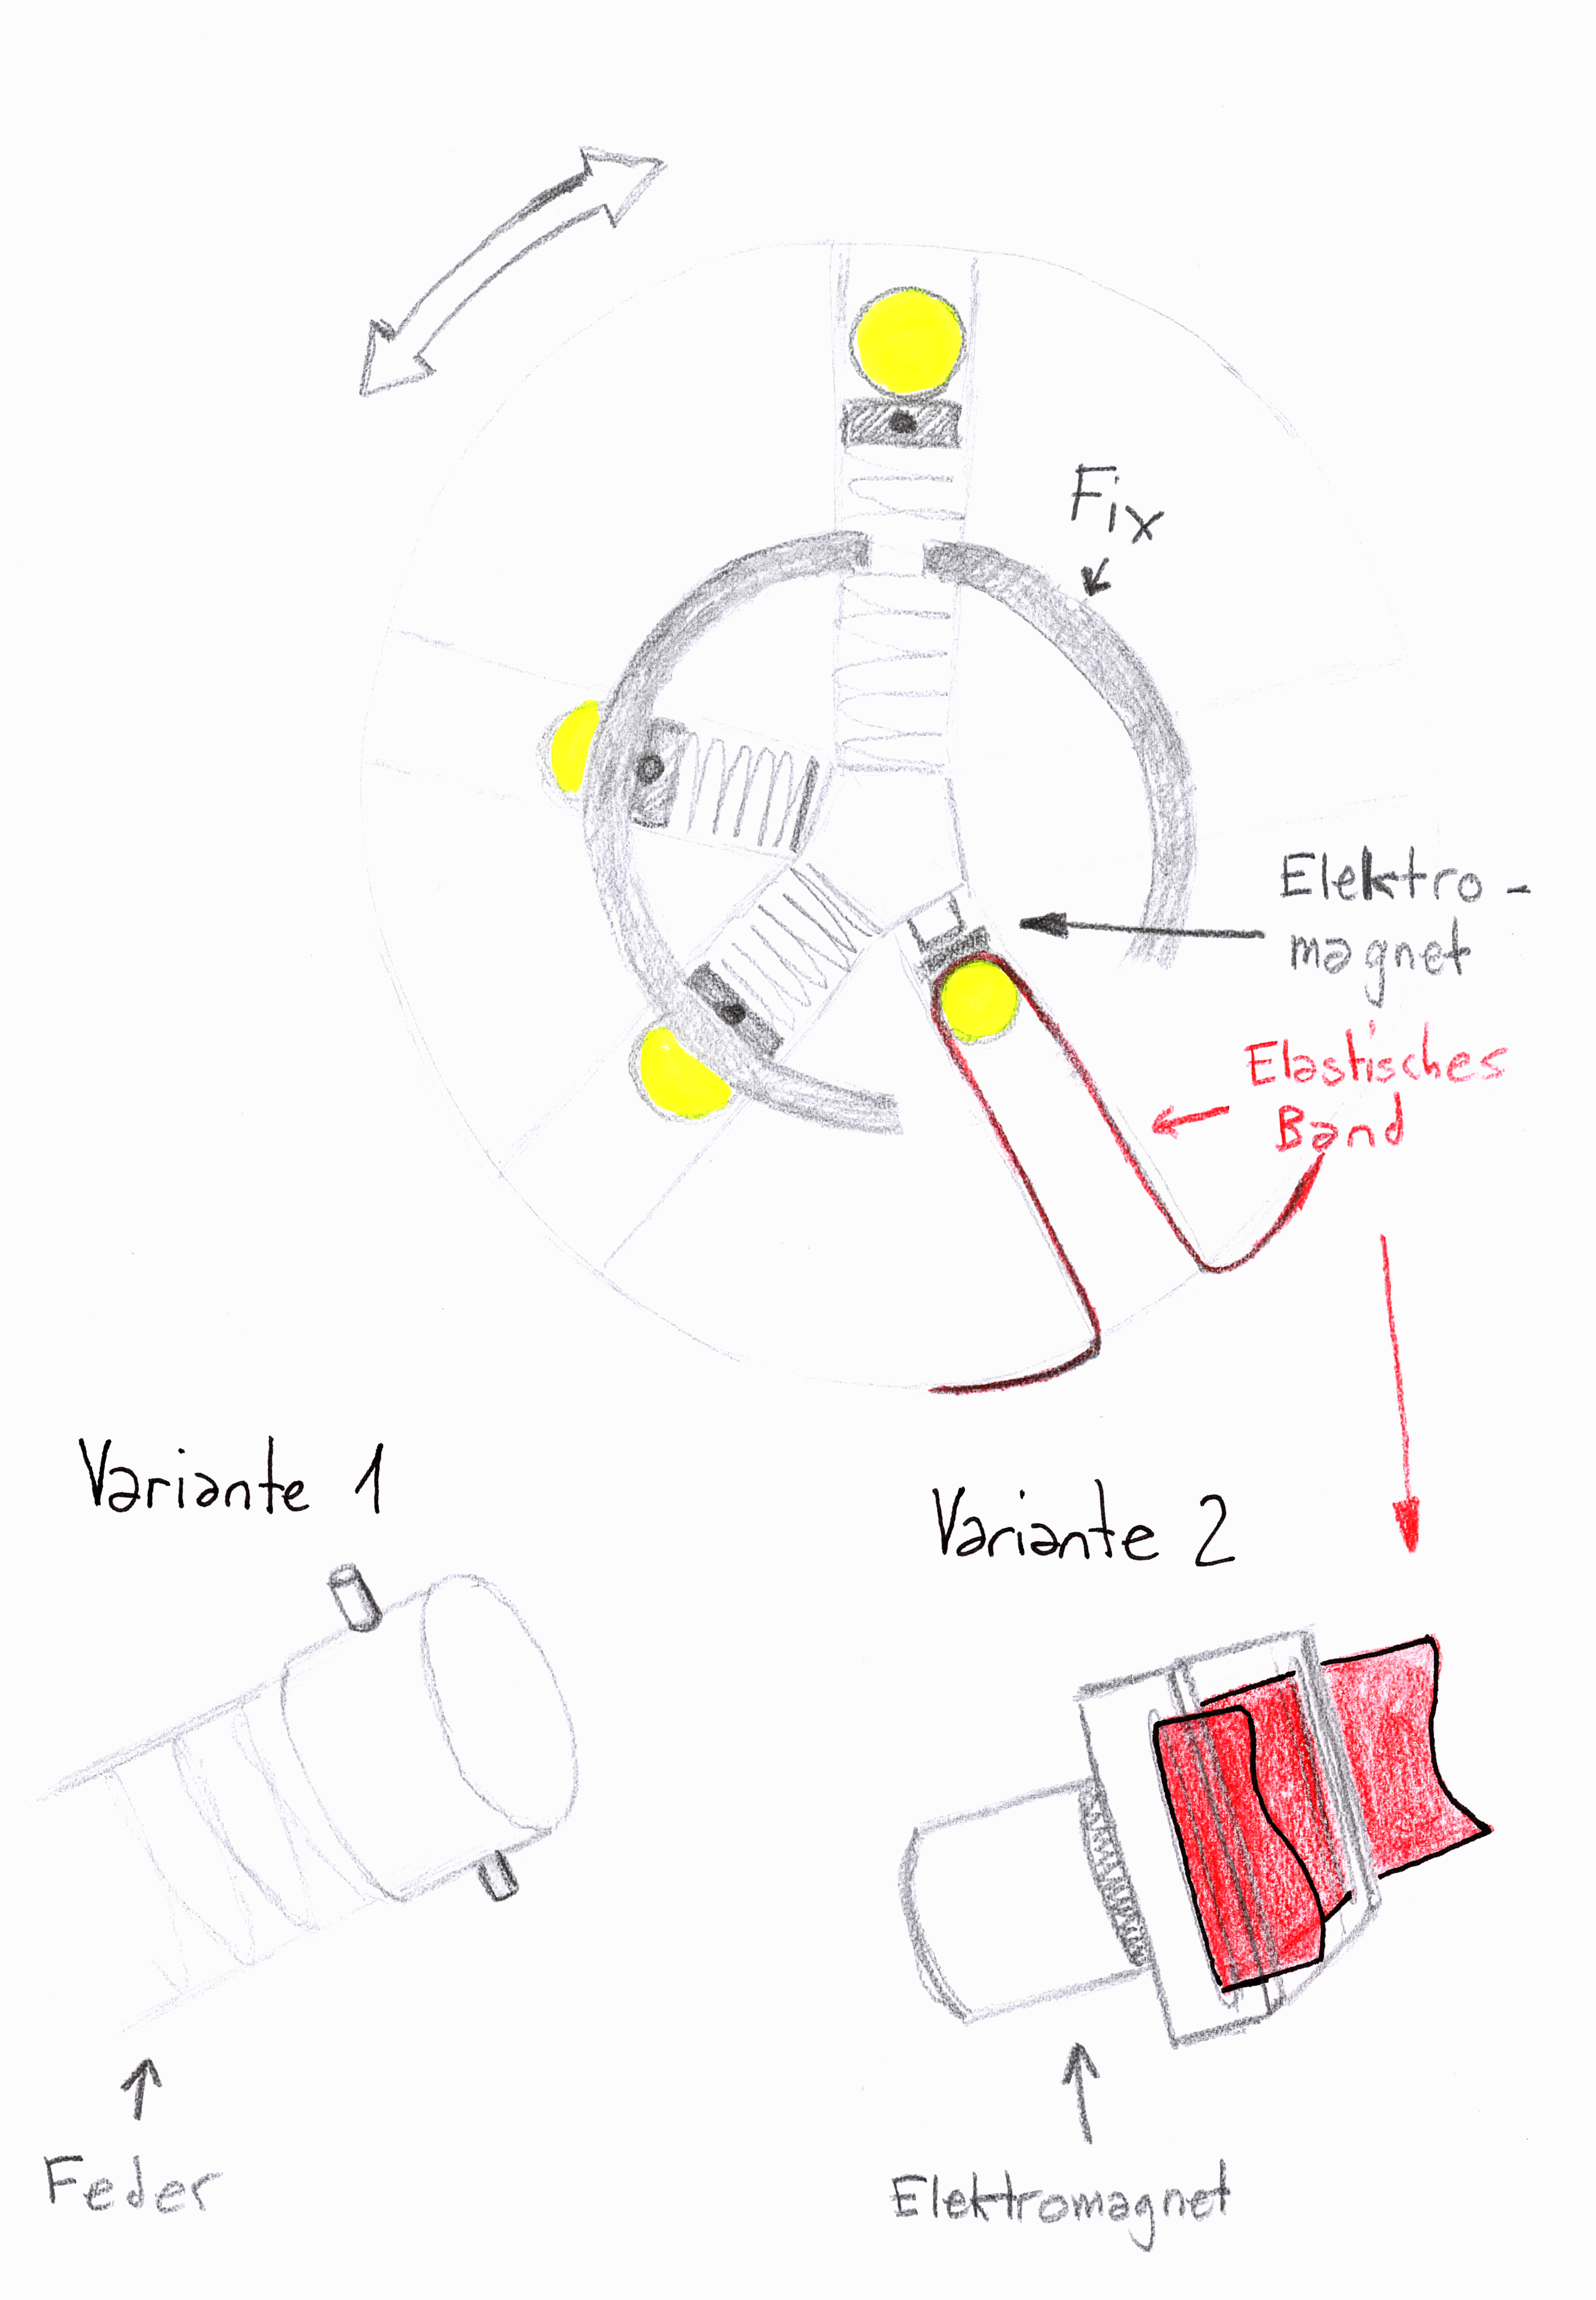
\includegraphics[width=0.4\textwidth]{../../fig/Feder_Gummirad.jpg}
	\caption{Rotierender Federbeschleuniger}
	\label{fig:feder_gummirad}
\end{figure}
Anders als bei den meisten bisherigen Ideen wird bei der fünften Idee auf ein Nachladeprozess verzichtet. Dies ist möglich, weil für jeden Ball ein beschleunigendes Element (Feder oder Gummiband) schon vorgespannt vorliegt. Für den ersten Ball wird die Vorrichtung ausgerichtet und für jeden weiteren Ball dann nur noch gedreht.

\subsection{Idee 6}
\begin{figure}[h!]
	\centering
	\includegraphics[width=0.5\textwidth]{../../fig/Fallrohr.jpg}
	\caption{Fallrohr}
	\label{fig:fallrohr}
\end{figure}
Diese Idee bedient sich der Schwerkraft als Beschleuniger. Die Bälle werden aus einer Höhe fallen gelassen und einer Führung entlang Richtung Korb gelenkt.

\subsection{Idee 7}
\begin{figure}[h!]
	\centering
	\includegraphics[width=0.5\textwidth]{../../fig/EM-Katapult.jpg}
	\caption{Katapult}
	\label{fig:katapult}
\end{figure}
Bei der siebten Idee werden die Bälle durch ein Katapult in den Korb geworfen. Das Katapult würde durch ein Elektromagnet in Wurfposition gehalten.

\subsection{Idee 8}
\begin{figure}[h!]
	\centering
	\includegraphics[width=0.5\textwidth]{../../fig/Elektrozylindergeraet.jpg}
	\caption{Elektrozylinder}
	\label{fig:elektrozylinder}
\end{figure}
Die achte Idee beinhaltet einen elektrischen Zylinder, der durch schnelles ausfahren jeweils einen Ball beschleunigt.
